\chapter{Ray tracing}\label{chap:raytracing}
Ray tracing is a geometric problem that describes the transport of light within optical systems.
It uses single rays to describe the propagation of light through an optical system.
The influence of diffraction on the transport of a ray is neglected and geometrical modeling of an optical system is considered.
Generally, the method can be implemented for two or more dimensions and for any optical system.
In the following a description of the ray tracing method is given. We restrict ourselves to two-dimensional case.
The two-dimensional case is particularly relevant because it is a good test case to demonstrate the performance of the new ray tracing method.
Optical designers often start with 2D systems where only the meridional plane is taken into account because it gives a good prediction of the target distribution of the rays
(see \cite{winston2005nonimaging}, chapter $4$, p.$50-65$). However, the two-dimensional case also has some limitations, as it may not identify skew rays that are turned back by the system, and so a 2D analysis cannot guarantee a proper treatment of non meridional rays in 3D. Hence, the 2D target intensity distribution is not exactly equal to the corresponding 3D intensity. Furthermore in this chapter we consider systems where only reflection and refraction are taken into account.
\section{Ray tracing for two-dimensional optical systems}\label{sec:raytracing}
Ray tracing is a procedure that can be applied to non-imaging systems. It consists of tracing each ray, which is considered to be a broken line, through the optical system.
Given a Cartesian coordinate system $(\variabile{x}, \variabile{z})$, a two-dimensional optical system symmetric with respect to the $\variabile{z}$-axis is defined.
Hence, usually the optical axis coincides with the $\variable{z}$-axis.
The optical system is formed by a source \point{S}, a target  \point{T} and some optical components $\lineai$ where $\lineai \in \{2, \cdots, \nline-1\}$ and $\nline$
 indicates the number of lines that form the system. \point{S} and \point{T} are indicated with the indexes $1$ and $\nline$, respectively.
The index of refraction of the medium in which line $\lineai$ is located is indicated with $\n_\lineai$
Every ray emitted by \point{S} (line $1$) can hit some optical components $\lineai\in\{2, \cdots, \nline -1\}$ before reaching \point{T} (line $\nline$).
The intersection point of the rays with line $\lineai$ are $(\variabile{x}_\lineai, \variabile{z}_\lineai)_{\lineai =1, \cdots, \nline}$ and, $\vect{s}_\lineai= (-\sin \optangle_\lineai, \cos \optangle_\lineai)$ indicates the direction vector of the rays that leave $\lineai$,
with $\optangle_\lineai$ the angle that the ray forms with respect to the optical axis measured counterclockwise. As we consider only forward rays, the angles
$\optangle_\lineai\in (-\pi/2, \pi/2)$.
Therefore, a ray segment between $(\variabile{x}_\lineai, \variabile{z}_\lineai)$ and $(\variabile{x}_\lineaj, \variabile{z}_\lineaj)$
with $\lineaj\neq\lineai$ is parameterized in real space by:
\begin{equation}
\label{parametrization}
\vect{r}(\variabile{s})=
\left( \begin{array}{cc}
\variabile{x}_\lineai-\variabile{s}\sin\optangle_\lineai \\
\variabile{z}_\lineai+\variabile{s}\cos\optangle_\lineai\end{array} \right) \qquad \quad 0< \variabile{s}\leq \variabile{s}_{\textrm{max}}\,,
\end{equation}
where \variabile{s} denotes the arc-length and $\variabile{s}_{\textrm{max}}$ is the maximum value that it can assume.
Fig. \ref{fig:cup} shows an example where a single ray is traced inside a very simple optical system, the so-called two-faceted cup.
\begin{figure}[h]
\label{fig:cup}
  \begin{center}
\vspace{-1.5cm}
  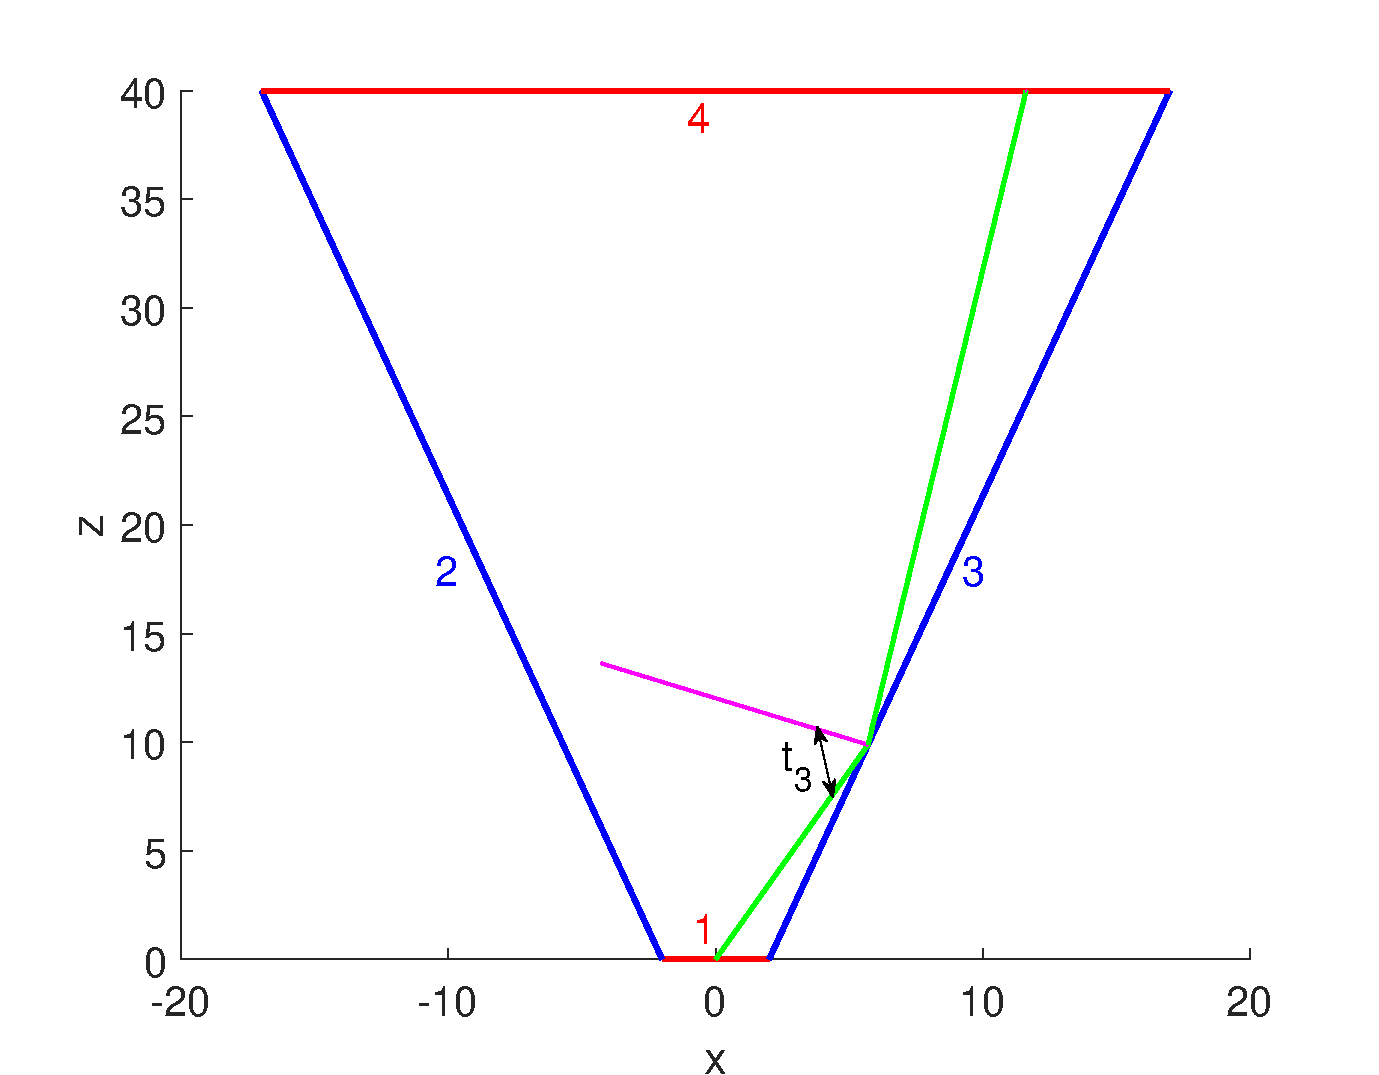
\includegraphics[width=6.7cm]{cup.pdf}
  \end{center}
\vspace{-2cm}
  \caption{\footnotesize{Shape of the two-faceted cup.  Each line of the system is labeled with a number.
   The source \point{S}$= [-2,2]$ (line number $1$) is located on the $\variabile{x}$-axis.
   The target \point{T}$= [-17, 17]$ (line $4$) is parallel to the source and is located at a height $\variabile{z}= 40$.
   The left and right reflectors (line $2$ and $3$) connect the source with the target.}}
  \label{fig:cup}
\end{figure}
The light source \point{S}$= [-\variabile{a}, \variabile{a}]$ (line $1$) and the target \point{T}$~=~ [-\variabile{b}, \variabile{b}]$ (line $4$) are two segments normal to the \variabile{z}-axis, where $\variabile{a}=2$ and $\variabile{b}=17$.
The left and right reflectors (line $2$ and $3$) are oblique segments that connect the source and the target.
All the optical lines $\lineai \in \{1, \cdots, 4\}$  are located in air, therefore the refractive index $\n_{\lineai}=1$ for every $\lineai$. \\ \indent
In order to compute the target photometric variables, we need to know how the optical system influences the direction of the rays when they hit an optical line.
 To this purpose, the ray tracing procedure is often used in optics.
Ray tracing relates the position coordinates
 $ (\variabile{x}_1, \variabile{z}_1)$ and the direction vector $\vect{s}_1$ of every ray at the source $\point{S}$ with the corresponding position $(\variabile{x}_\nline, \variabile{z}_\nline)$ and direction $\vect{s}_\nline$
 at the target $\point{T}$. As in the following we will use often the target coordinates of the rays, from now on, to simplify the notation, we write $(\variabile{x},\variabile{z})$ instead of $(\variabile{x}_\nline, \variabile{z}_\nline)$,  $\optangle$ instead of $\optangle_\nline$ and $\vect{s}$ instead of $\vect{s}_{\nline}$ for the target coordinates.
The ray tracing algorithm can be schematized as follows.
\begin{enumerate}
 \item[1. ] Given a ray that leaves $\point{S}$ with initial position $(\variabile{x}_1, \variabile{z}_1)$ and initial direction $\vect{s}_1~=~(-\sin \optangle_1, \cos \optangle_1)$, use Eq. ($\ref{parametrization}$) to implement the ray parametrization $\vect{r}(\variabile{s}_1)$;
\item[2. ] Compute the coordinates $(\variabile{x}_\variabile{k}, \variabile{z}_\variabile{k})_{\variabile{k} = 1\cdots, \nline}$ of the intersection point of the ray with all the lines that it hits;
\begin{itemize}
\item[a)] If the shape of the lines is described by equations with a known analytical description, the intersection points are determined analytically;
\item[b)] If there is no analytic description for the optical lines, the intersections need to be determined using iterative methods;
\end{itemize}
\item  Computing the minimum of the distances between the previous ray's position coordinates $(\variabile{x}_1, \variabile{z}_1)$ and the coordinates $(\variabile{x}_\variabile{k}, \variabile{z}_\variabile{k})$ for every ${\variabile{k} = 1\cdots, \nline}$ and determine the closest line $\lineai$ that the forward ray encounters;
\item If $\lineai = \nline$ stop the procedure, the target ray's coordinates $(\variabile{x}, \variabile{z})$ and $\vect{s}$ are found.
\item Calculate the normal $\boldsymbol{\nu}_\variabile{i}$ to line $\variabile{i}$ at the point $(\variabile{x}_{\variabile{i}}, \variabile{z}_{\variabile{i}})$;
 \item Compute the new ray direction $\vect{s}_\lineai$ of the ray that leaves line $\lineai$ at the point $(\variabile{x}_{\variabile{i}}, \variabile{z}_{\variabile{i}})$;
\begin{itemize}
\item[a)] If the incident line is a reflective line, $\vect{s}_\lineai$ is given by Eq. (\ref{Reflection});
\item[b)] If the incident line is a refractive line, $\vect{s}_\lineai$ is given by Eq. (\ref{Refraction});
\end{itemize}
\item Restart the procedure from $1.$ for the ray that leaves line $\lineai$ instead of \point{S}. Consider as initial ray position coordinates $(\variabile{x}_{\variabile{i}}, \variabile{z}_{\variabile{i}})$ instead of $(\variabile{x}_1, \variabile{z}_1)$ and as initial ray direction $\vect{s}_\lineai= (-\sin \optangle_\lineai, \cos \optangle_\lineai)$ instead of $\vect{s}_1$.
\end{enumerate}
The procedure explained above is repeated for every ray traced through the system, \cite{Gross2005Handbook}. There are different ways to implement the ray tracing procedure.
An often used method is MC ray tracing which is explained in the next paragraph.
\section{Monte Carlo ray tracing}
%Say that MC methods are used to calculate an integral
%\begin{figure}[h]
%\label{fig:cup}
%  \begin{center}
%
%  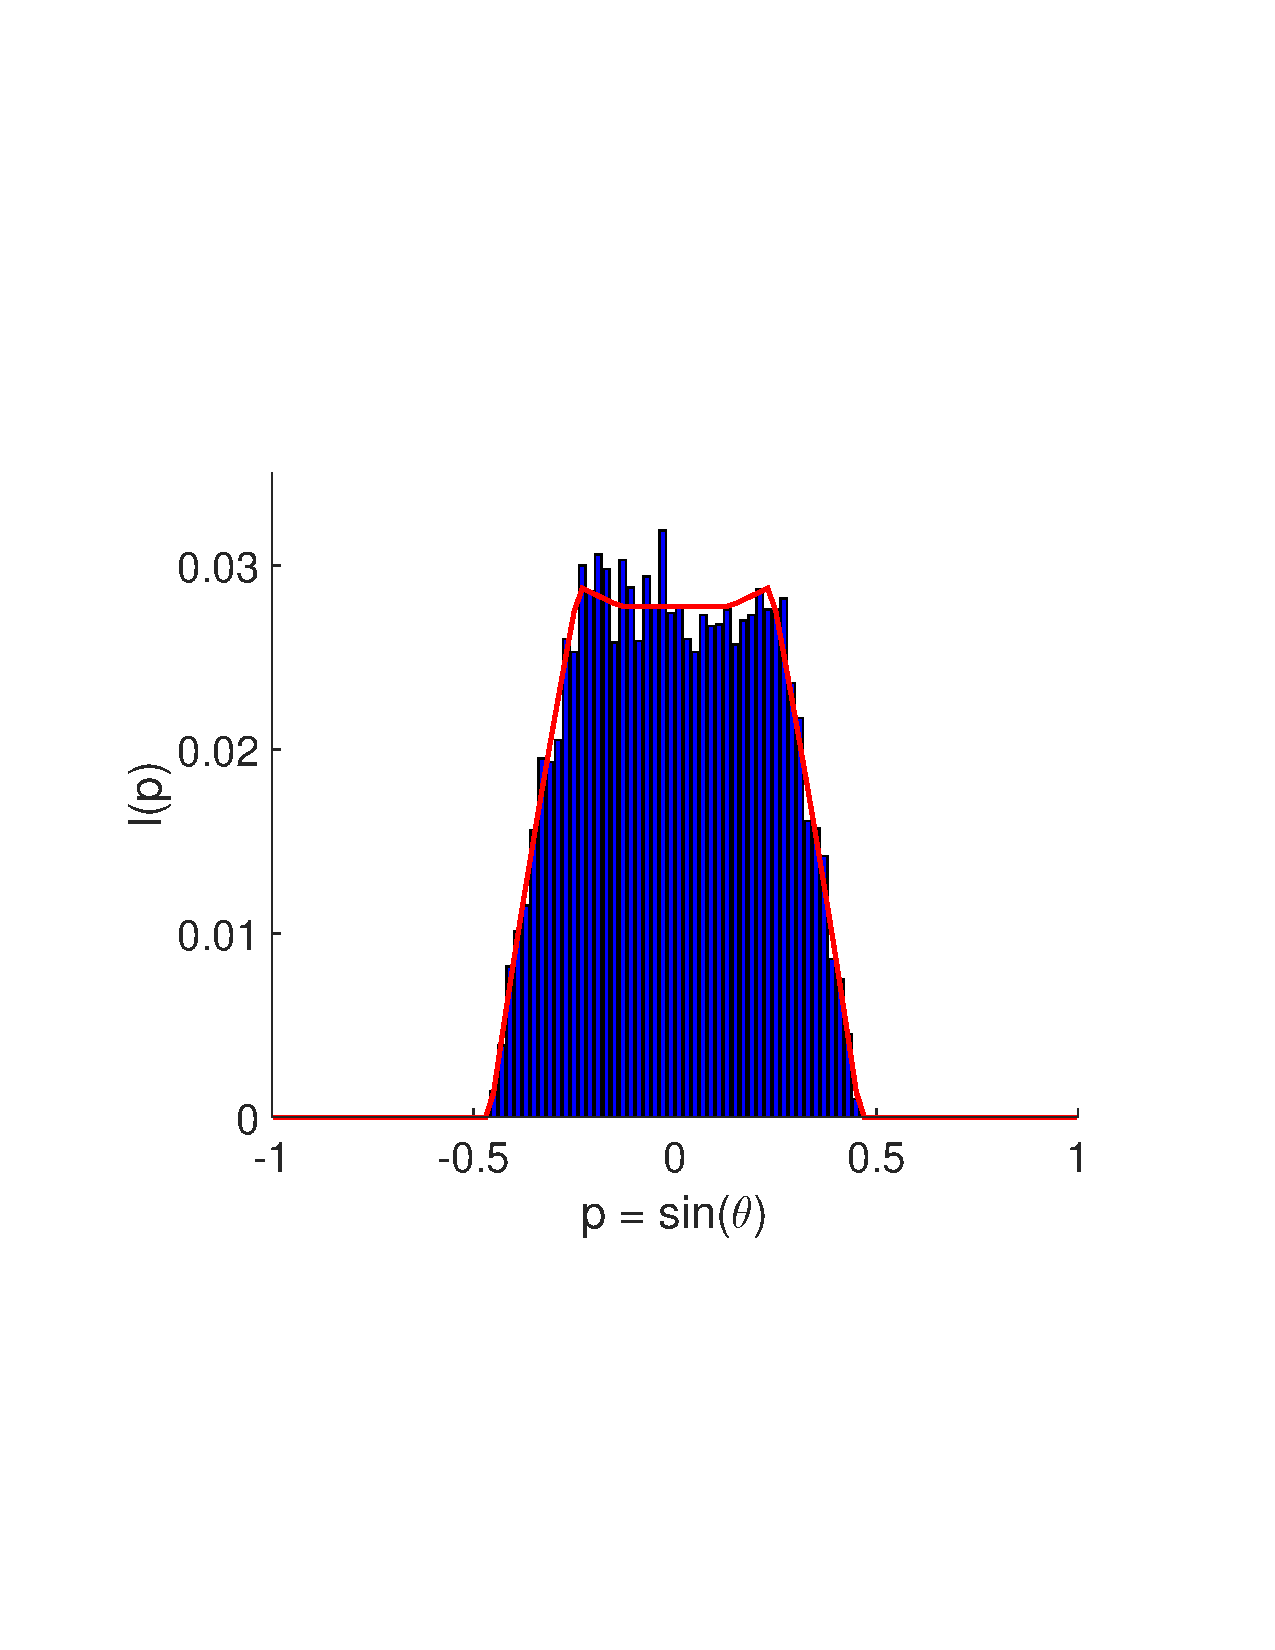
\includegraphics[width=10cm]{MC_raytracing.pdf}
%  \end{center}
%\vspace{-2cm}
%  \caption{\footnotesize{Shape of the two-faceted cup.  Each line of the system is labeled with a number.
%   The source \point{S}$= [-2,2]$ (line number $1$) is located on the $x$-axis.
%   The target \point{T}$= [-17, 17]$ (line $4$) is parallel to the source and is located at a height $z= 40$.
%   The left and right reflectors (line $2$ and $3$) connect the source with the target.}}
%  \label{fig:cup}
%\end{figure}
%\begin{figure}[h]
%\label{fig:cup}
%  \begin{center}
%
%  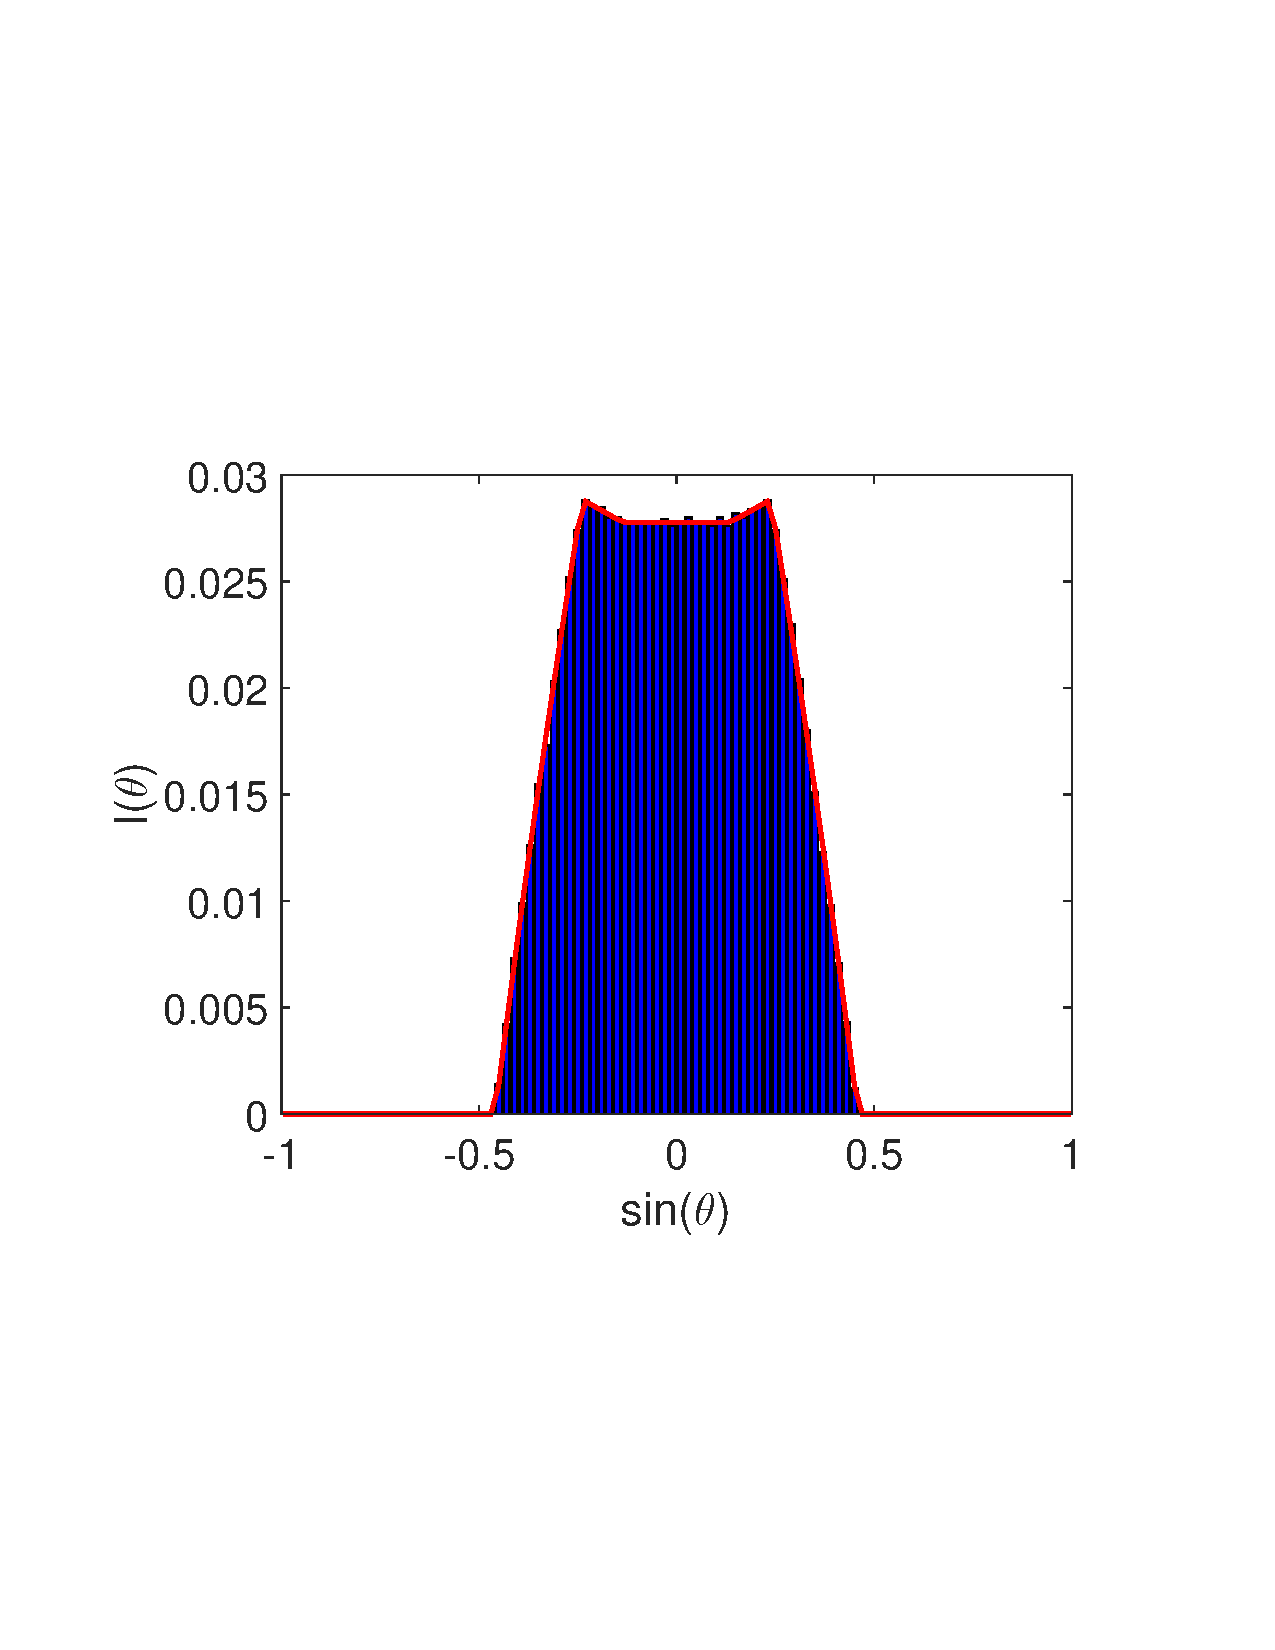
\includegraphics[width=10cm]{qmc_raytracing.pdf}
%  \end{center}
%\vspace{-2cm}
%  \caption{\footnotesize{Shape of the two-faceted cup.  Each line of the system is labeled with a number.
%   The source \point{S}$= [-2,2]$ (line number $1$) is located on the $x$-axis.
%   The target \point{T}$= [-17, 17]$ (line $4$) is parallel to the source and is located at a height $z= 40$.
%   The left and right reflectors (line $2$ and $3$) connect the source with the target.}}
%  \label{fig:cup}
%\end{figure}

% Intensity integral of the luminance
% Luminance constant
Before explain MC ray tracing procedure we give a general introduction about MC methods. MC simulation are often used to approximate the integral of a given function $f$ considering random variables in the domain of $f$. More precisely, given a function $f:[a,b]^d\subseteq \mathbb{R}^d \mapsto \mathbb{R}$ and a random variable $\variabile{y}\in D = [a, b]^d$ with probability density function $\rho(\variabile{y})$, the expected value of $f$ is defines as:
\begin{equation}
\variabile{E}[f] =\int_{D}f(\variabile{y})\rho(\variabile{y}) \textrm{d}\variabile{y}.
\end{equation}
Note that if $\rho$ is a uniform probability density function, we have:
\begin{equation}
\variabile{E}[f] = \int_{D}f(\variabile{y})\rho(\variabile{y}) \textrm{d}\variabile{y} =\frac{1}{(b-a)^d} \int_{D}f(\variabile{y}) \textrm{d}\variabile{y}.
\end{equation}
In Monte Carlo methods $\const{N}$ independent random variables  $\variabile{y}_1, \cdots, \variabile{y}_{\const{N}}$  from the density $\rho$ are considered and, the sum
\begin{equation}
S_{\const{N}}(f) = \frac{1}{\const{N}} \sum_{\variabile{i}=1}^{\textrm{N}} f(\variabile{y}_\variabile{i})
\end{equation}
is calculated,  \cite{owen2003quasi}.
The strong law of large numbers tells us that:
\begin{equation}
\const{Pr}\Big(\lim_{\const{N}\rightarrow\infty}\sum_{\variabile{i}=1}^{\const{N}} f(\variabile{y}_\variabile{i}) = \variabile{E}[f(\variabile{y})] \Big) = 1.
\end{equation}
Therefore the following relation holds:
\begin{equation}
\variabile{E}[f] \approx \frac{1}{\const{N}} \sum_{\variabile{i}=1}^{\const{N}} f(\variabile{y}_\variabile{i}).
\end{equation}
Suppose that $f$ has variance $Var[f]=\sigma^2[f] $, then
\begin{equation}
Var[S_\const{N}(f)] = \variabile{E}[(S_{\const{N}}(f)-\variabile{E}[S_{\const{N}}(f)])^2]= \variabile{E}[(S_{\const{N}}(f)-\variabile{E}[S_{\const{N}}(f)])^2] = \sigma^2/\const{N}
\end{equation}
where the second equality follows from the linearity of the expected value:
\begin{equation}
\variabile{E}[S_{\const{N}}(f)] = \frac{1}{\const{N}}\sum_{\variabile{i}=1}^{\textrm{N}}\variabile{E}[ f(\variabile{y}_\variabile{i})].
\end{equation}
Indicating the integration error with:
\begin{equation}
\const{err}(f, S_{\const{N}}) =\int_{D}f(\variabile{y})\rho(\variabile{y}) \textrm{d}\variabile{y}-\frac{1}{\const{N}}S_{\const{N}}(f)
\end{equation}
we obtain that
\begin{equation}\label{eq:mean_error}
\variabile{E}\big[|\const{err}(f, S_{\const{N}})|\big]\leq\sqrt{\variabile{E}\big[\const{err}(f, S_{\const{N}})^2\big]} = \frac{\sigma[f]}{\sqrt{\const{N}}}.
\end{equation}
Hence, the absolute value of the integration error is, on average, bounded by $\sigma[f]/\sqrt{\const{N}}$, where $\sigma[f]$ is the standard deviation of function $f$, \cite{leobacher2014introduction}. It is worthy to note that $\const{err}(f, S_{\const{N}})$ does not depend on the dimension $d$ of function $f$.
\\ \indent MC technique can be combined with the ray tracing procedure in order to compute the light distribution at the target of an optical system.
Monte Carlo ray tracing is based on this idea and, it is explained in the following.
MC ray tracing uses as sample of random variables a set of points the coordinates of which correspond to the position and direction coordinates of every ray at the source of the optical system.
Therefore, rays with a random initial position and a random initial direction are traced from \point{S} to \point{T} within the optical system.
In this way a probabilistic interpretation of the output photometric variables is provided.
In particular, we are interested in the total target intensity $I$ which is computed as a function of the angular coordinate $\optangle$.
The MC intensity is calculated dividing the target into intervals of the same length, the so-called bins. A partitioning
$P_1: -\pi/2 = \optangle_{0}<\optangle_{1}<\cdots <\optangle_{\const{Nb}}=\pi/2$ of the interval $[-\pi/2, \pi/2]$ is defined where $\const{Nb}$ is the number of bins in $P_1$.
We remark that, with a slight abuse of notation, we indicated the angular coordinates of the rays at the target (line $\nline$) with $\optangle_{\variabile{j}}$ instead of $\optangle_{\nline,\variabile{j}}$ for every $\variabile{j}\in\{0, \cdots, \const{Nb}\}$.
The normalized approximated intensity $I_{\const{MC}}(\optangle)$ is a piecewise constant function and its value over the $\variabile{j}$-th bin is the ratio between the number of rays that fall into that bin
$\const{Nr}[\optangle_{\variabile{j}-1},\optangle_{\variabile{j}})$ and the total number of rays traced $\const{Nr}[-\pi/2, \pi/2]$.
Hence, $I_{\const{MC}}$ is defined by:
\begin{equation} \label{g_mc}
I_{\const{MC}}(\optangle) = \frac{\const{Nr}[\optangle_{\variabile{j}-1},\optangle_{\variabile{j}})}{\const{Nr}[-\pi/2, \pi/2]} \qquad \mbox{ for } \optangle\in[\optangle_{\variabile{j}-1}, \optangle_{\variabile{j}}).
\end{equation}
Furthermore, the output intensity is computed from the value of the intensity $I_{\const{MC}}(\optangle_{\variabile{j}-1/2})$ along the direction $\optangle_{\variabile{j}-1/2}=(\optangle_{\variabile{j}-1}+
\optangle_{\variabile{j}})/2$ for every bin $[\optangle_{\variabile{j}-1},\optangle_{\variabile{j}})_{\variabile{j} = 1, \cdots, \const{Nb}}$.
 The intensity $I_{\const{MC}}(\optangle_{\variabile{j}-1/2})$ gives an estimate of the probability that a ray reaches the target with an angle in the $\variabile{j}$-th interval
$[\optangle_{\variabile{j}-1}, \optangle_{\variabile{j}})$ of the partitioning $P_1$. This probability $\const{P}_{\variabile{j}, \Delta\optangle}$ is given by:
\begin{equation}\label{eq:probability}
\const{P}_{\variabile{j}, \Delta\optangle} = \Pr(\optangle_{\variabile{j}-1}\leq\optangle<\optangle_{\variabile{j}})=
\frac{\int_{\optangle_{\variabile{j}-1}}^{\optangle_{\variabile{j}}} I(\optangle) \textrm{d}\optangle}{\int_{-\pi/2}^{\pi/2}I(\optangle) \textrm{d}\optangle}\,,
\end{equation}
where $I(\optangle)$ is the output intensity (not normalized) and it is measured in lumen per radian $[\textrm{lm}/\textrm{rad}]$.
Note that $\sum_{\variabile{j}=1}^{\const{Nb}}\const{P}_{\variabile{j}, \Delta\optangle}=1$. Using the mean value theorem for the function
$I(\optangle)$ continuous in $[\optangle_{\variabile{j}-1}, \optangle_{\variabile{j}}]$, the integral at the numerator of the previous equation can be written as: \begin{equation}
\int_{\optangle_{\variabile{j}-1}}^{\optangle_{\variabile{j}}} I(\optangle) \textrm{d}\optangle = \Delta \optangle\;I(\optangle_{j-1/2}).
\end{equation}
Hence, $\const{P}_{\variabile{j}, \Delta\optangle}$ is proportional to the size $\Delta\optangle= (\optangle_{\const{Nb}}-\optangle_{0})/{\const{Nb}}$
of the intervals, i.e., inversely proportional to the number of bins $\const{Nb}$ of the partitioning $P_1$.
Indicating with $\Phi = \int_{-\pi/2}^{\pi/2}I(\optangle) \textrm{d}\optangle$ the total flux (measured in lumen $[\textrm{lm}]$),
the error between the intensity $I(\optangle_{\variabile{j}-1/2})$
 and the averaged \const{MC} intensity $\Phi I_{\const{MC}}(\optangle_{\variabile{j}-1/2})/\Delta\optangle$ is given by:
\begin{equation}\label{eq:error_int}
\begin{aligned}
\Big|I(\optangle_{\variabile{j}-1/2})&-\frac{\Phi}
{\Delta\optangle}I_{\const{MC}}(\optangle_{\variabile{j}-1/2})\Big| \leq\\
 &\Big|I(\optangle_{\variabile{j}-1/2})-\frac{1}{\Delta \optangle}\int_{\optangle_{\variabile{j}-1}}^{\optangle_{\variabile{j}}} I(\optangle)\textrm{d}\optangle\Big|+\\
&\frac{1}{\Delta \optangle}\Big|\int_{\optangle_{\variabile{j}-1}}^{\optangle_{\variabile{j}}} I(\optangle)\textrm{d}\optangle-
\Phi\, I_{\const{MC}}(\optangle_{\variabile{j}-1/2})\Big| \,.
\end{aligned}
\end{equation}
\indent The first term of the right hand side of inequality (\ref{eq:error_int}) gives an estimate of how much the averaged intensity
 $\frac{1}{\Delta \optangle}\int_{\optangle_{\variabile{j}-1}}^{\optangle_{\variabile{j}}} I(\optangle)\textrm{d}\optangle$ differs from the exact intensity $I(\optangle_{\variabile{j}-1/2})$.
This term is due to the discretization of the target and therefore it depends on the number of bins $\const{Nb}$ considered.
  Substituting $I(\optangle)$ with its Taylor expansion around the point $\optangle_{\variabile{j}-1/2}$ we obtain that this term is proportional to the square of the size of the bins, therefore the following equality holds:
\begin{equation}\Big|I(\optangle_{\variabile{j}-1/2})-\frac{1}{\Delta \optangle}\int_{\optangle_{\variabile{j}-1}}^{\optangle_{\variabile{j}}} I(\optangle)\textrm{d}\optangle\Big| = \const{C}_1/\const{Nb}^2\end{equation}
with $C_1>0$ a certain constant. \\
\indent
The second part of the right hand side of inequality (\ref{eq:error_int}) gives an estimate of the MC error and therefore it depends also on the
number of rays traced.
In order to show how this term decreases as a function of the number of rays traced,
we define the random variable $\variabile{X}_\variabile{j}(\optangle)$ as the variable that is equal to $1$ if the ray with angular coordinate $\optangle$
is inside the interval $[\optangle_{\variabile{j}-1}, \optangle_{\variabile{j}})$ and equal to $0$ otherwise,
\begin{equation}
\label{radom_variable}
\variabile{X}_{\variabile{j}}(\optangle) = \begin{cases} \begin{aligned}
1& \qquad \mbox{if} \quad \optangle\in [\optangle_{\variabile{j}-1}, \optangle_{\variabile{j}}),\\
0 & \qquad \mbox{otherwise}.
\end{aligned}\end{cases}
\end{equation}
The Bernoulli trial $ \variabile{X}_{\variabile{j}}$ follows a binomial distribution $B(1,\const{P}_{\variabile{j}, \Delta\optangle})$.
Considering a sample of $\const{Nr}$ rays, the variable $\variabile{Y}_{\variabile{j}} = \sum_{\variabile{k}=1}^{\const{Nr}} \variabile{X}_{\variabile{j}}(\optangle_{\variabile{k}})$
follows a binomial distribution $B(\const{Nr}, \const{P}_{\variabile{j},\Delta \optangle})$, where $\optangle_{\variabile{k}}$ is the angle that the $\variabile{k}$-th ray forms
 with the optical axis. Then, using the de Moivre-Laplace theorem, we conclude that the variable $\variabile{Y}_{\variabile{j}}$ is approximated by a normal distribution with mean value
$\variabile{E}[\variabile{Y}_{\variabile{j}}] = \const{Nr}\const{P}_{\variabile{j}, \Delta\optangle}$ and variance $\sigma^2[\variabile{Y}_{\variabile{j}}] = \const{Nr}\const{P}_{\variabile{j}, \Delta\optangle}(1~-~\const{P}_{\variabile{j}, \Delta\optangle})$
when a large number of rays is considered, see \cite{zolotarev1997modern, rubinstein2016simulation}.
Thus, the normalized intensity along the direction $\optangle_{\variabile{j}-1/2}$ is given by:
\begin{equation}I_{\const{MC}}(\optangle_{\variabile{j}-1/2}) = \sum_{\variabile{k}=1}^{\const{Nr}}\variabile{X}_{\variabile{j}}(\optangle_{\variabile{k}})/\const{Nr}.\end{equation}
The mean value $E[I_{\const{MC}}(\optangle_{\variabile{j}-1/2})]=\const{P}_{\variabile{j}, \Delta\optangle}$
and the variance $\sigma^2[I_{\const{MC}}(\optangle_{\variabile{j}-1/2})] ~=~ \const{P}_{\variabile{j}, \Delta\optangle}(1-\const{P}_{\variabile{j}, \Delta\optangle})/\const{Nr}$.
Note that the standard deviation $\sigma_\variabile{j}:=\sigma[I_{\const{MC}}(\optangle_{\variabile{j}-1/2})]$ equals:
\begin{equation}\label{sigma}
\sigma_\variabile{j}= \sqrt{\const{P}_{\variabile{j}, \Delta\optangle}(1-\const{P}_{\variabile{j}, \Delta\optangle})/\const{Nr}}= \frac{\const{C}_2}{\sqrt{\const{Nb}\const{Nr}}}\,, \end{equation}
 for some $\const{C}_{2}>0$. $\sigma_\variabile{j}$ can be used to give an estimate of the difference between the intensity $I_{\const{MC}}(\optangle_{\variabile{j}-1/2})$ and its mean value $\const{P}_{\variabile{j}, \Delta\optangle}$.
Therefore, the second term of the right hand side of relation ($\ref{eq:error_int}$) becomes:
\begin{equation}\begin{aligned}
\frac{1}{\Delta \optangle}\Big|\int_{\optangle_{\variabile{j}-1}}^{\optangle_{\variabile{j}}} I(\optangle)\textrm{d}\optangle -
\Phi\, I_{\const{MC}}(\optangle_{\variabile{j}-1/2})\Big| &=  \\
\frac{\Phi}{\Delta \optangle}\Big|\const{P}_{\variabile{j}, \Delta\optangle} -I_{\const{MC}}(\optangle_{\variabile{j}-1/2})\Big| &\propto  \\
  \frac{\Phi}{\Delta \optangle}
\sigma_{\variabile{j}}[I_{\const{MC}}(\optangle_{\variabile{j}-1/2})]=\const{C}_3\frac{\const{Nb}}{\sqrt{\const{Nb}\const{Nr}}} & = \const{C}_3\sqrt{\frac{\const{Nb}}{\const{Nr}}}\,,
\end{aligned}
\end{equation}
for some $\const{C}_3>0$, where the approximation holds because $\sigma_{\variabile{j}}$ gives a measure for the error between
$I_{\const{MC}}(\optangle_{\variabile{j}-1/2})$ and the probability $\const{P}_{\variabile{j}, \Delta\optangle}$, \cite{diez2012openintro}. The second equality follows from Eq. (\ref{sigma}). To conclude, the MC error over the $\variabile{j}$-th bin is estimated by:
\begin{equation} \begin{aligned}
\Big|I(\optangle_{\variabile{j}-1/2})&-\frac{\Phi}
{\Delta\optangle}I_{\const{MC}}(\optangle_{\variabile{j}-1/2})\Big| =
\frac{\const{C}_1}{\const{Nb}^2} + \const{C}_4\sqrt{\frac{\const{Nb}}{\const{Nr}}},
\end{aligned}
\end{equation}
for $\const{C}_4>0$.
Considering a fixed number of rays, we obtain that the minimal error is reached when $\const{Nb}\approx \const{Nr}^{1/5}$.
Hence, if $10^{10}$ rays are considered the target has to be divided into $10^2$ bins to minimize the MC error.
This leads to computational efforts resulting in a very slow procedure.\\ \indent
To give an example we implemented MC ray tracing for the two-faceted cup the profile of which is depicted in Fig. \ref{fig:cup}.
A set of random rays with coordinates $(\variabile{x}_{\variabile{k}}, \optangle_{\variabile{k}})_{\variabile{k}= 1, \cdots, \const{Nr}}$ is generated at the source. We considered for instance $\const{Nr}=10^4$ rays. The rays distribution on the $(\variabile{x}_{\variabile{k}}, \optangle_{\variabile{k}})$-plane is shown in Fig. \ref{fig:mc_sample}.
\begin{figure}[h]
\begin{center}
    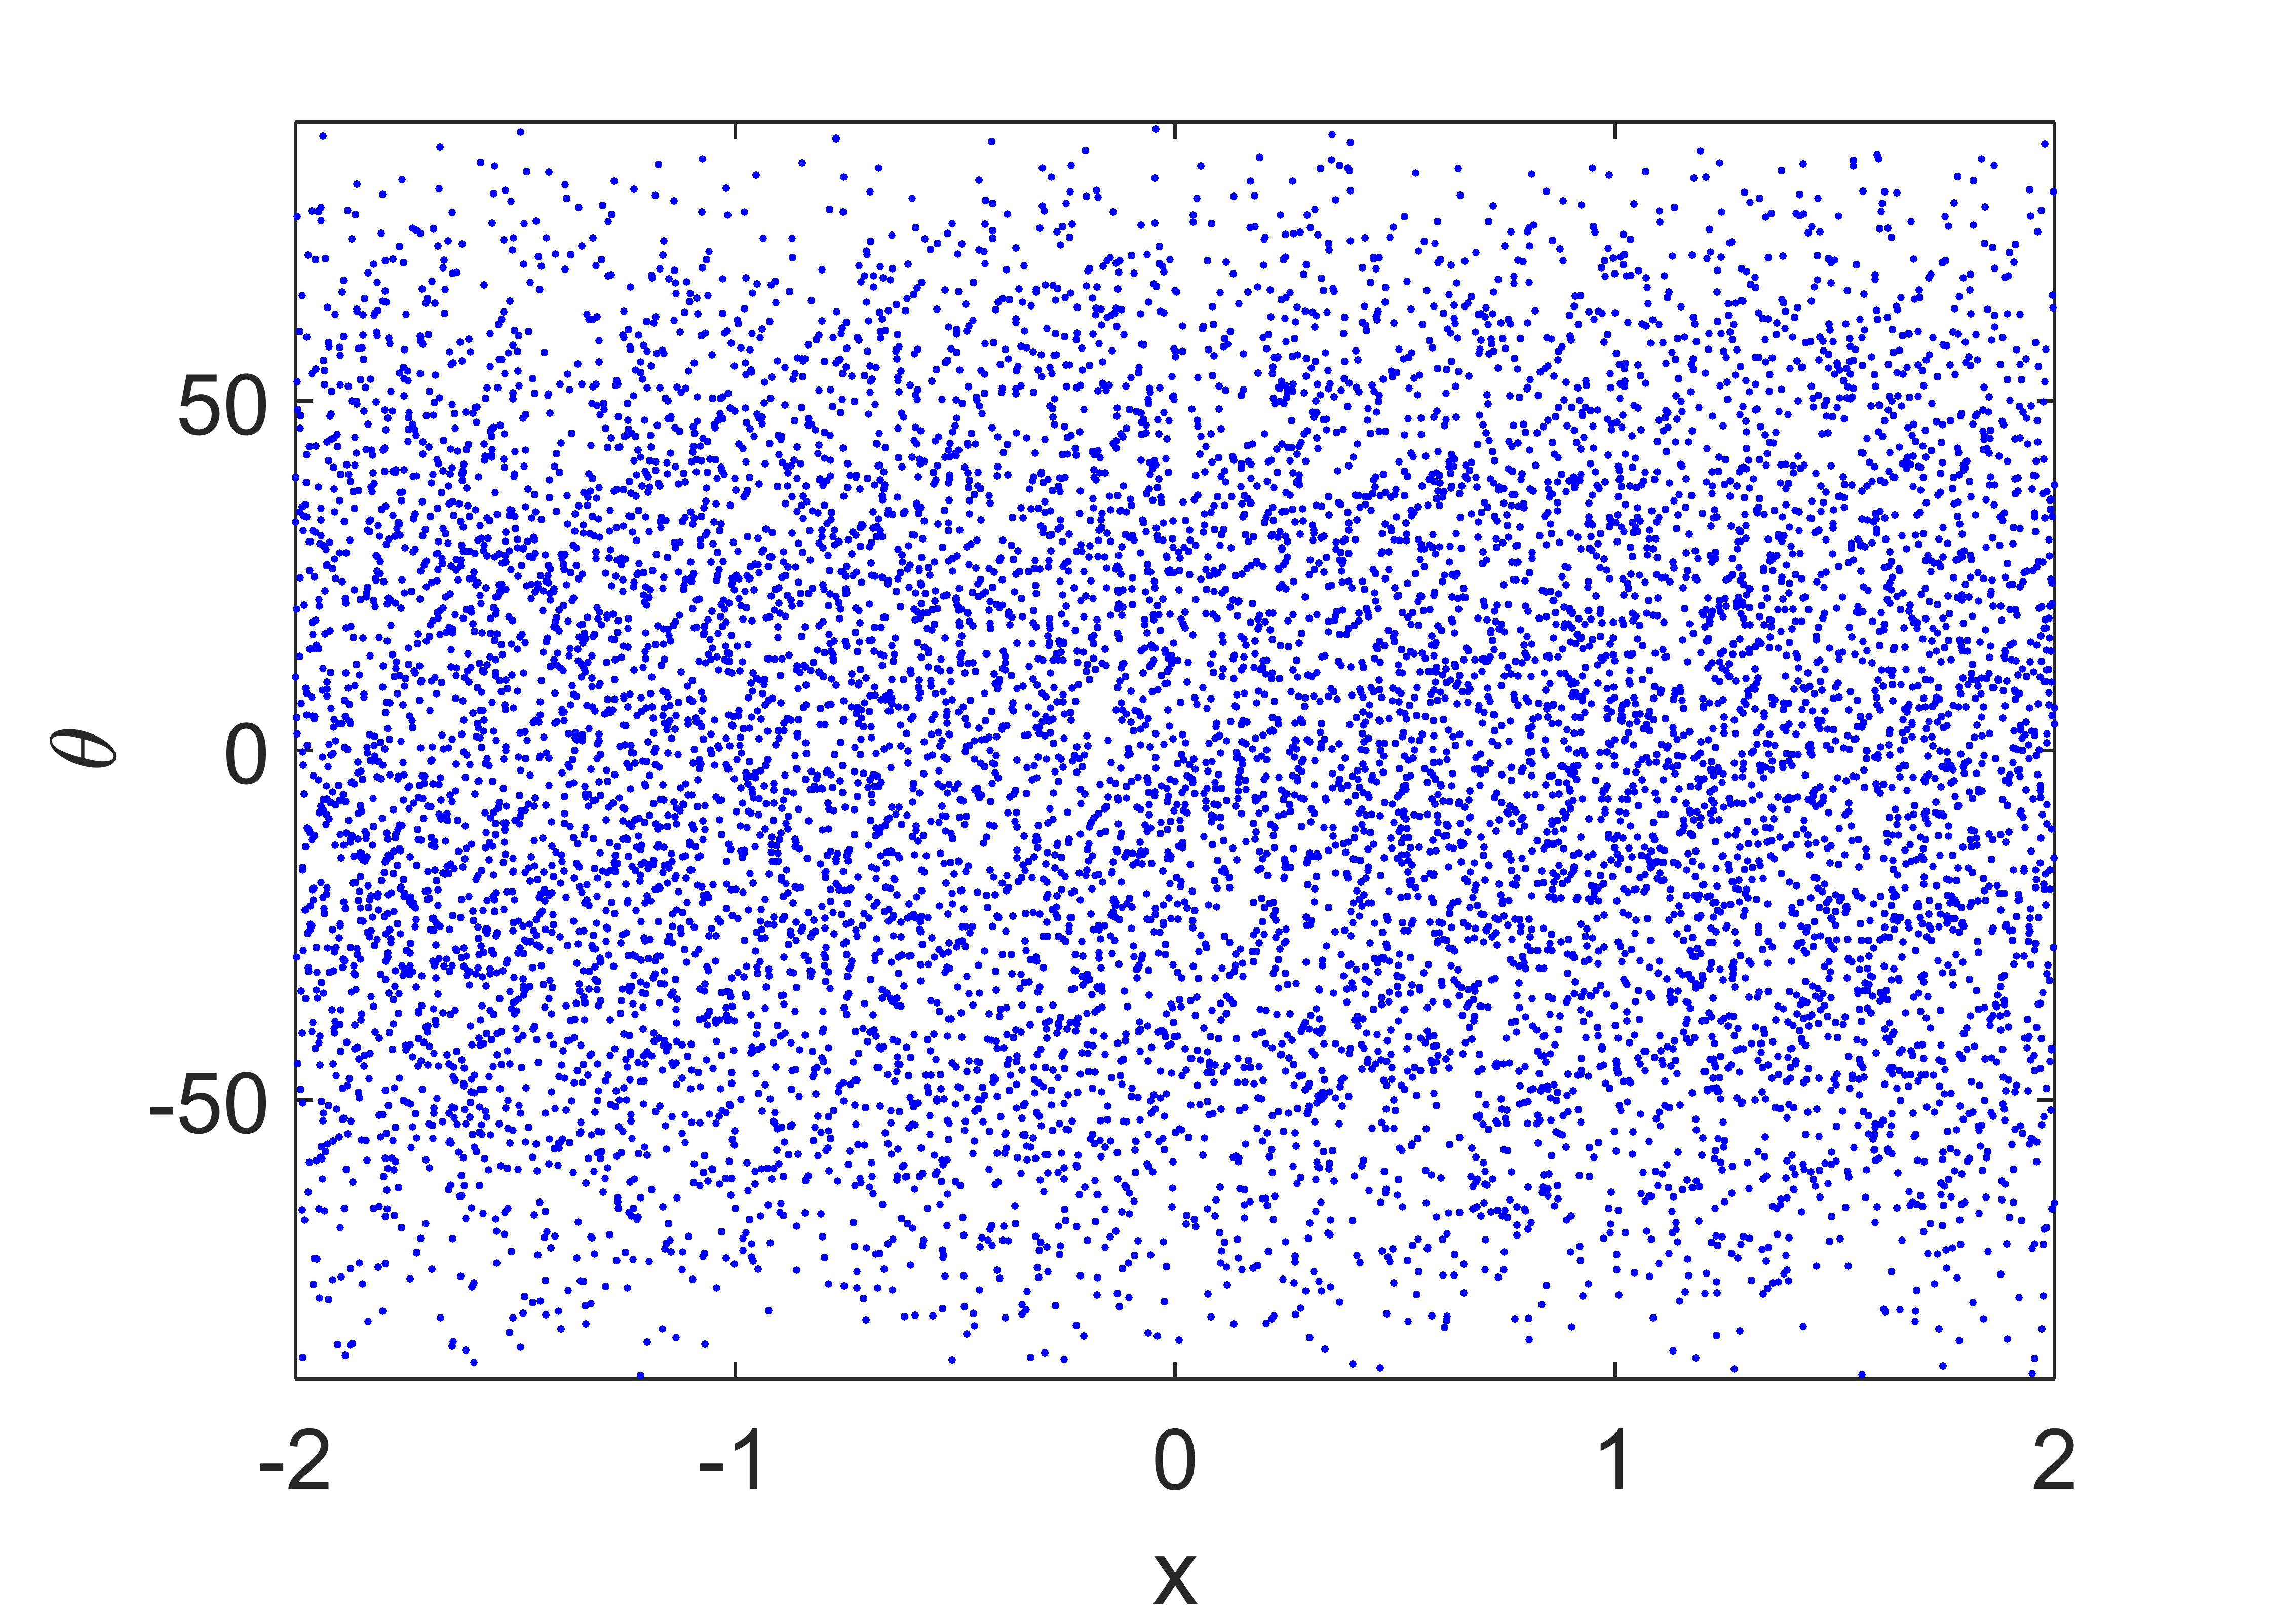
\includegraphics[width=0.8\textwidth]{mc_sample.jpg}
    \caption{Rays at the source of the two-faceted cup with random position coordinate $\variabile{x}$ and random angular coordinates $\optangle$. $10^4$ rays are depicted in this figure.}
    \label{fig:mc_sample}
\end{center}
  \end{figure}
Every sample ray is traced inside the system using the ray tracing procedure. Then, the target $\point{T} = [-\variabile{b}, \variabile{b}]$ is divided into $\const{Nb}= 100$ bins.
Using Eq. (\ref{g_mc}), the normalized intensity $I_{\const{MC}}$ is computed. $I_{\const{MC}}$  is a piecewise constant function, therefore the averaged normalized intensity  $\hat{I}_{\const{MC}}(\optangle_{\variabile{j}-1/2})= \frac{1}{\Delta \optangle}I_{\const{MC}}(\optangle_{\variabile{j}-1/2})$ is given considering the values that the intensity  $I_{\const{MC}}$ assumes on the middle point $(\optangle_{\variabile{j}-1/2})_{\variabile{j} = 0, \cdots, \const{Nb}}$ of every bin. The profile of $\hat{I}_{\const{MC}}$ is depicted in Fig. \ref{fig:mc_raytrancing_intensity} with the red line. The exact intensity $I$ (analytic intensity) is shown with the green line in the same figure.
\begin{figure}[t]
\begin{center}
    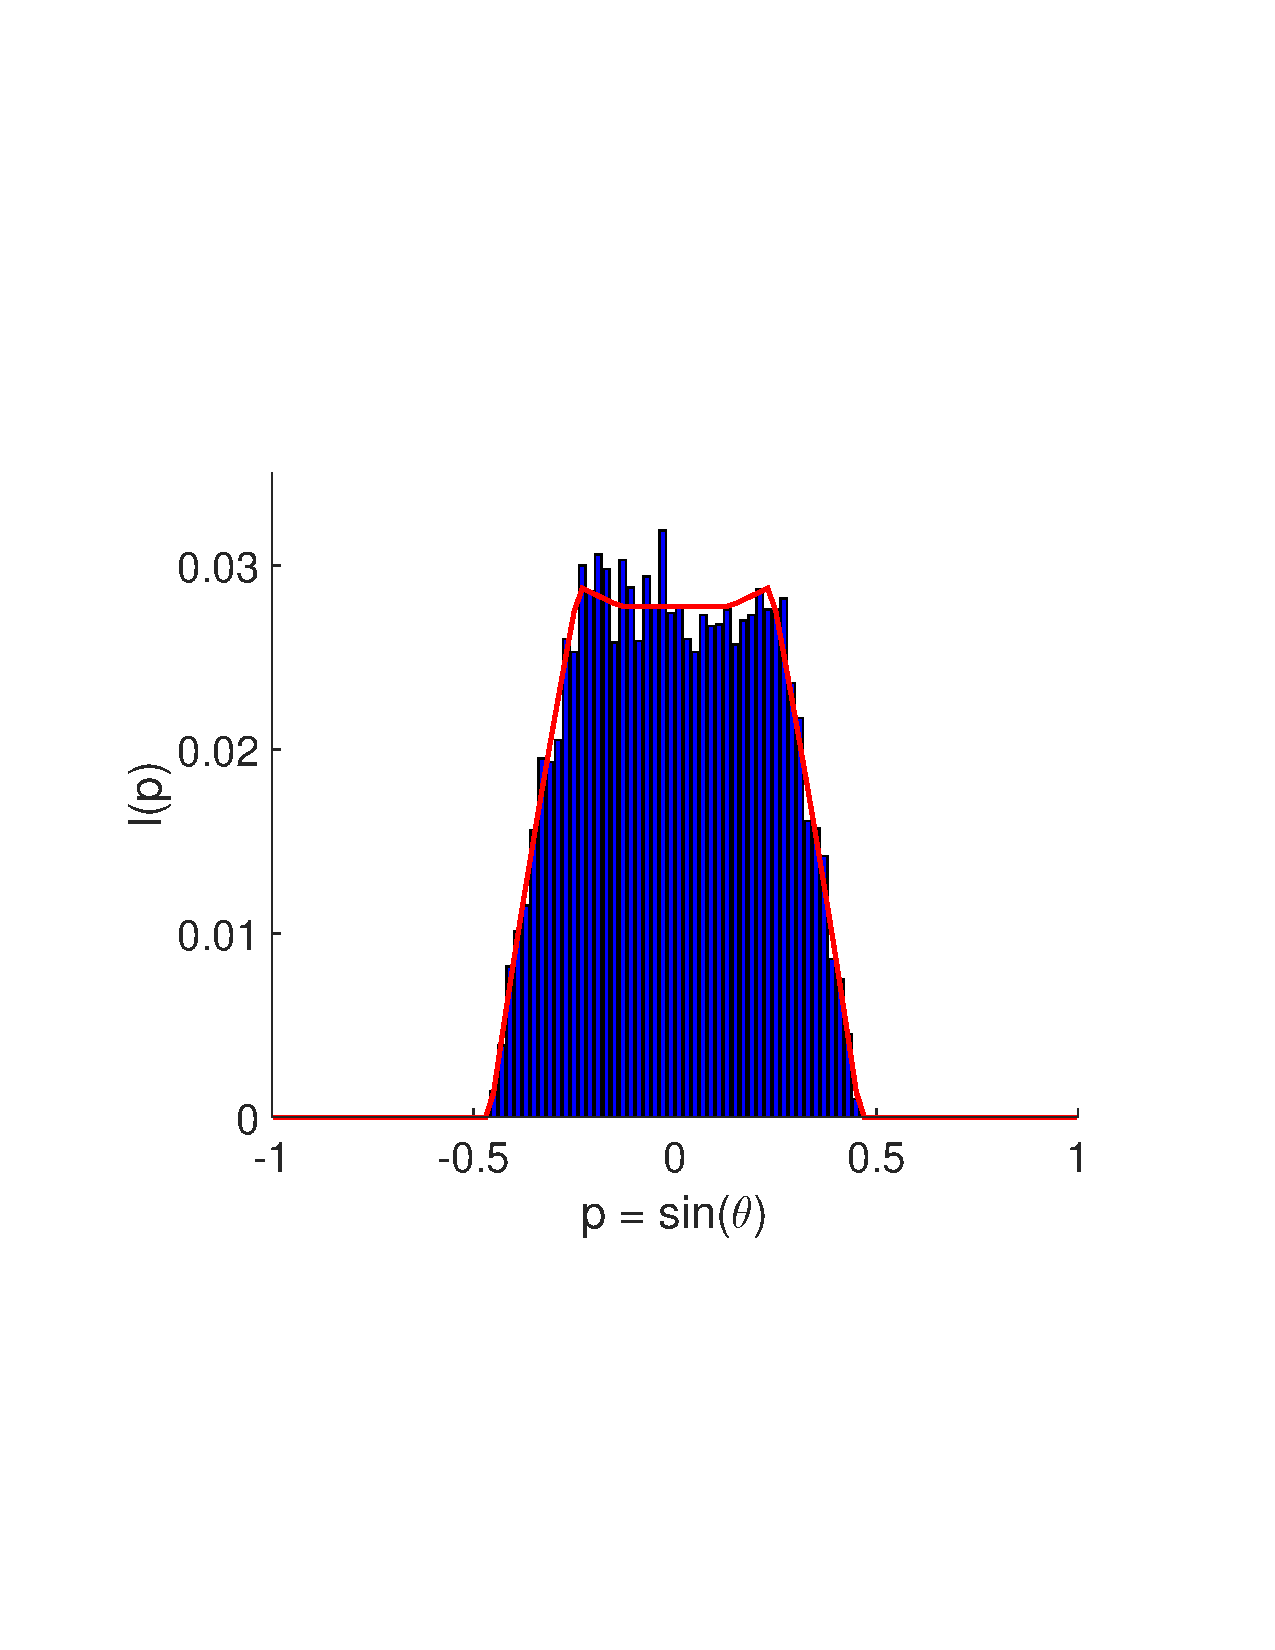
\includegraphics[width=0.8\textwidth]{MC_raytracing.jpg}
    \caption{Comparison between the averaged normalized MC intensity and the normalized exact intensity.}
   \label{fig:mc_raytrancing_intensity}
\end{center}
\end{figure}
From Fig. \ref{fig:mc_raytrancing_intensity} it is obvious that $10^4$ ray are not enough to have a good intensity's approximation and a big effect of noise is still observed.
\\ \indent
To conclude, MC ray tracing has the advantages of being very easy to implement and it does not require too much regularity of the function that has to be approximate. Furthermore, the error convergence does not depend on the dimension of the domain in which the function is defined.
On the other hand, MC method is time consuming as the error has a speed of convergence of the order $(1/\sqrt{\const{N}})$. Furthermore, MC ray tracing is a binning procedure, therefore the error depends also on the number of bins in which the target is divided. Finally, it is a statistical procedure and the error bound is only a "probabilistic" error as shown in Eq. (\ref{eq:mean_error}). This means that, to calculate the value of the error, several simulations have to be repeated and the average of the errors obtained in every simulation has to be calculated. \\ \indent MC ray method can be improved using a deterministic approach.
Instead of considering random variables $\variabile{y}_1, \cdots, \variabile{y}_{\const{N}}$, a sample of points can be defined in such a way that they have a regular distribution on the domain $D\subseteq[a,b]^d$ of the function $f$ of which we want to compute the integral. Methods based on this deterministic approach are called Quasi Monte Carlo (QMC) methods.
\section{Quasi-Monte Carlo ray tracing}
Quasi-Monte Carlo (QMC) methods were proposed for the first time in the 1950s in order to deal with the issues encountered in MC.
Likewise MC methods, QMC procedures can be used to approximate the integral of a function.
The idea is to generate a set of points $\point{y}_1, \cdots, \point{y}_\const{N}$ which are not random distributed but also not exactly uniformly distributed, \cite{}.
To measure how much the distribution of these points differs from a uniform distribution, the concept of discrepancy was introduced.
Usually, discrepancy is restricted to intervals $[\point{a}, \point{b})\subseteq [0.1)^d$. Intuitively, discrepancy measures how much the samples differ from a uniform distribution.
Therefore, random sequences have a very high discrepancy, while uniform distributed sequences have zero discrepancy. There are different notions of discrepancies, one of the simplest is the star discrepancy:
 \begin{definition}
Let $\mathcal{S} = \{\point{y}_1, \cdots, \point{y}_\const{N}\}$ be a set of $\const{N}$ points in $[0,1)^d$. The  star discrepancy $D^*_\const{N}({\mathcal{S}})$ of $\mathcal{S}$ is defined as:
\begin{equation}
D^*_\const{N}({\mathcal{S}}) = \sup_{\point{a}\in[0,1)^d}\Big|\frac{1}{\const{N}}\sum_{\variabile{i} = 1}^{\const{N}}\chi_{[0,\point{a})}(\variabile{y}_\variabile{i})-\lambda_d([0, \point{a}))\Big|
\end{equation}
where $\chi_{[0,\point{a})}(\variabile{y}_\variabile{i})$ is the indicator function of $[0,\point{a})\subseteq [0.1)^d$ and $\lambda_d([0, \point{a})) = \prod_{\variabile{j}=1}^d \point{a}_\variabile{j}$ denotes the the $d$-dimensional Lesbegue measure. For intervals of the form $[\point{a}, \point{b})\subseteq [0.1)^d$ we have $\lambda_d([\point{a}, \point{b}))=\prod_{\variabile{j}=1}^{d}(\point{b}_\variabile{j}-\point{a}_\variabile{j})$.
\end{definition}
% Maybe add a picture
Sequences constructed such that the corresponding star discrepancy has an order of $O(\log(\const{N})^d/\const{N})$ are called \textit{low-discrepancy sequences}, \cite{owen2003quasi}.
There are many way to generate low discrepancies sequences.
We first show a particular construction for $d=1$ that was introduced the first time by Van der Corput in 1935.  This kind of sequences, called \textit{van der Corput} sequences, are particular interesting first of all because they give an intuition of how to construct low discrepancy sequences and, then, because many other kind of sequences in higher dimensions use this approach.
Let $\const{b}\geq 2$ be an integer base. Any natural number $\variabile{n}\in \mathbb{N}_0$ can be decomposed in base $\const{b}$ as follows:
\begin{equation}
\variabile{n} = \sum_{\variabile{i}=0}^\infty \variabile{d}_{\variabile{i}}\const{b}^{\variabile{i}}
\end{equation}
where $\variabile{d}_{\variabile{i}} \in \{0, 1, \cdots, \const{b}-1\}$ are the so-called the digit numbers.
The radical inverse function $\phi_{\const{b}}(\variabile{n})$ in base $\const{b}$ is defined as:
\begin{equation}
\phi_{\const{b}}(\variabile{n}) = \sum_{\variabile{i}=1}^{\infty}\frac{\variabile{d}_{\variabile{i}-1}}{\const{b}^{\variabile{i}}}.
\end{equation}
As an example we provide in the following the radical inverse function $\phi_{\const{b}}(5)$ in base $\const{b} = 2$. The digit expansion in base $\const{b}$ of $\variabile{n}=5$ is:
\begin{equation}
5 = 1\cdot 2ˆ0+1\cdot 2ˆ2
\end{equation}
\begin{definition}
The Van der Corput sequence in base $\const{b}$ is defined as $(\variabile{y}_{\variabile{n}})_{n\in\mathbb{N}_0}$ with $\variabile{y}_{\variabile{n}} = \phi_{\const{b}}(\variabile{n})$.
\end{definition}


% Uniform distribution modulo one
% say something about Sobol low discrepances sequences
% Estimation for the error
% Application of QMC in optics
% Quasi Monte Carlo ray tracing
% Disadvantages of QMC
